\chapter{순물질의 물리적 변화}
    \section{순수한 물질의 상평형도}
        \begin{defn}[상(Phase)]
            화학적 조성과 물리적 상태가 일정한 물질의 형태를 \textbf{상(Phase)}이라 한다.
        \end{defn}
        즉 고체, 액체, 기체, 또는 고체의 여러 결정상 등을 일컫는다. 상의 개수를 $P$로 나타낸다. 기체 혼합물이나 완전히 혼합된 액체 혼합물의 상의 개수는 
        $P=1$이다. \textbf{섞이지 않는(Immiscible)} 두 상이 있을 경우 이를 $P=2$로 나타내고, \textbf{섞이는(Miscible)} 하나의 상일 경우  
        $P=1$로 나타낸다. 현탁액과 같은 \textbf{분산물(Dispersion)}의 경우, 상이 두 개이므로 $P=2$이다.
        \par \begin{defn}[상태 변화]
        \textbf{상태 변화(Phase transition)}는 한 상이 다른 상으로 바뀌는 자발적 과정이다.
        \end{defn}이는 \textbf{상태 변화 온도(Transition temperature, $T_\mathrm{trs}$)}에서 일어난다. 상태 변화 온도에서는 두 상이 평형 상태를 
        이루고, 정해진 압력에서 계의 Gibbs 에너지는 최소가 된다. 상태 변화는 주로 \textbf{열분석(Thermal analysis)}을 통해 
        확인한다. 만약 상태 변화가 발열 반응일 경우, 계의 에너지를 감소시키면서 측정하면 온도 변화가 없는 구간이 나타난다. 반대로 
        상태 변화가 흡열 반응일 경우, 계의 에너지를 증가시키면서 측정하면 마찬가지로 온도 변화가 없는 구간이 나타난다. 이를 통해 
        상태 변화를 측정한다. 주로 DSC(\ref{enthal}, \ref{thermalchem} 참조)와 X선 산란 분광법이 이용된다.
        \par \begin{defn}[준안정 상]
        주어진 압력에서 가장 안정하진 않으나, 상태 변화 속도가 매우 느려 다른 상태로 거의 변하지 않는 상을 
        \textbf{준안정 상(Metastable phase)}이라 한다.
        \end{defn}
        예를 들어 다이아몬드는 흑연에 비해 1 bar에서 에너지가 높지만, 상태 
        변화에 필요한 활성화 에너지가 너무 높기 때문에 다이아몬드는 준안정 상에 해당한다.
        \par 상태 변화가 일어나기 위해서는 다음과 같은 조건을 만족해야 한다:
        \begin{rem}[상태 변화의 조건]
            평형 상태에서 물질의 화학적 퍼텐셜은 계에 있는 모든 상에 대해 같다. 
        \end{rem}
        A상과 B상이 평형을 이룬다고 할 때, A의 화학적 퍼텐셜 $\mu_\mathrm{A}$과 B의 화학적 퍼텐셜 $\mu_\mathrm{B}$에 대해 
        $\difform n$만큼 A에서 B로 변화할 때 화학적 퍼텐셜 변화는
        \begin{equation*}
            \difform G = -\mu_\mathrm{A} \difform n + \mu_\mathrm{B} \difform n = \left(\mu_\mathrm{B} - \mu_\mathrm{A}\right) \difform n
        \end{equation*}
        이다. 이 둘이 평형이므로, $\difform G = 0$이다. 따라서 $\mu_\mathrm{A} = \mu_\mathrm{B}$일 때 두 상(혹은 그 이상)이 평형을 
        이룬다.
        \par 순수한 물질의 \textbf{상평형도(Phase diagram)}는 주어진 압력과 온도에서 열역학적으로 안정한 상이 무엇인지 나타낸 그림이다. 
        상평형도에서 영역 사이의 선, 즉 \textbf{상 경계(Phase boundary)}에서는 두 상이 공존하며 평형을 이룬다. 즉 두 상의 화학적 퍼텐셜이 
        동일하다. 상평형도는 다음 Figure \ref{f5}과 같이 나타난다.
        \begin{figure}[H]
            \centering
            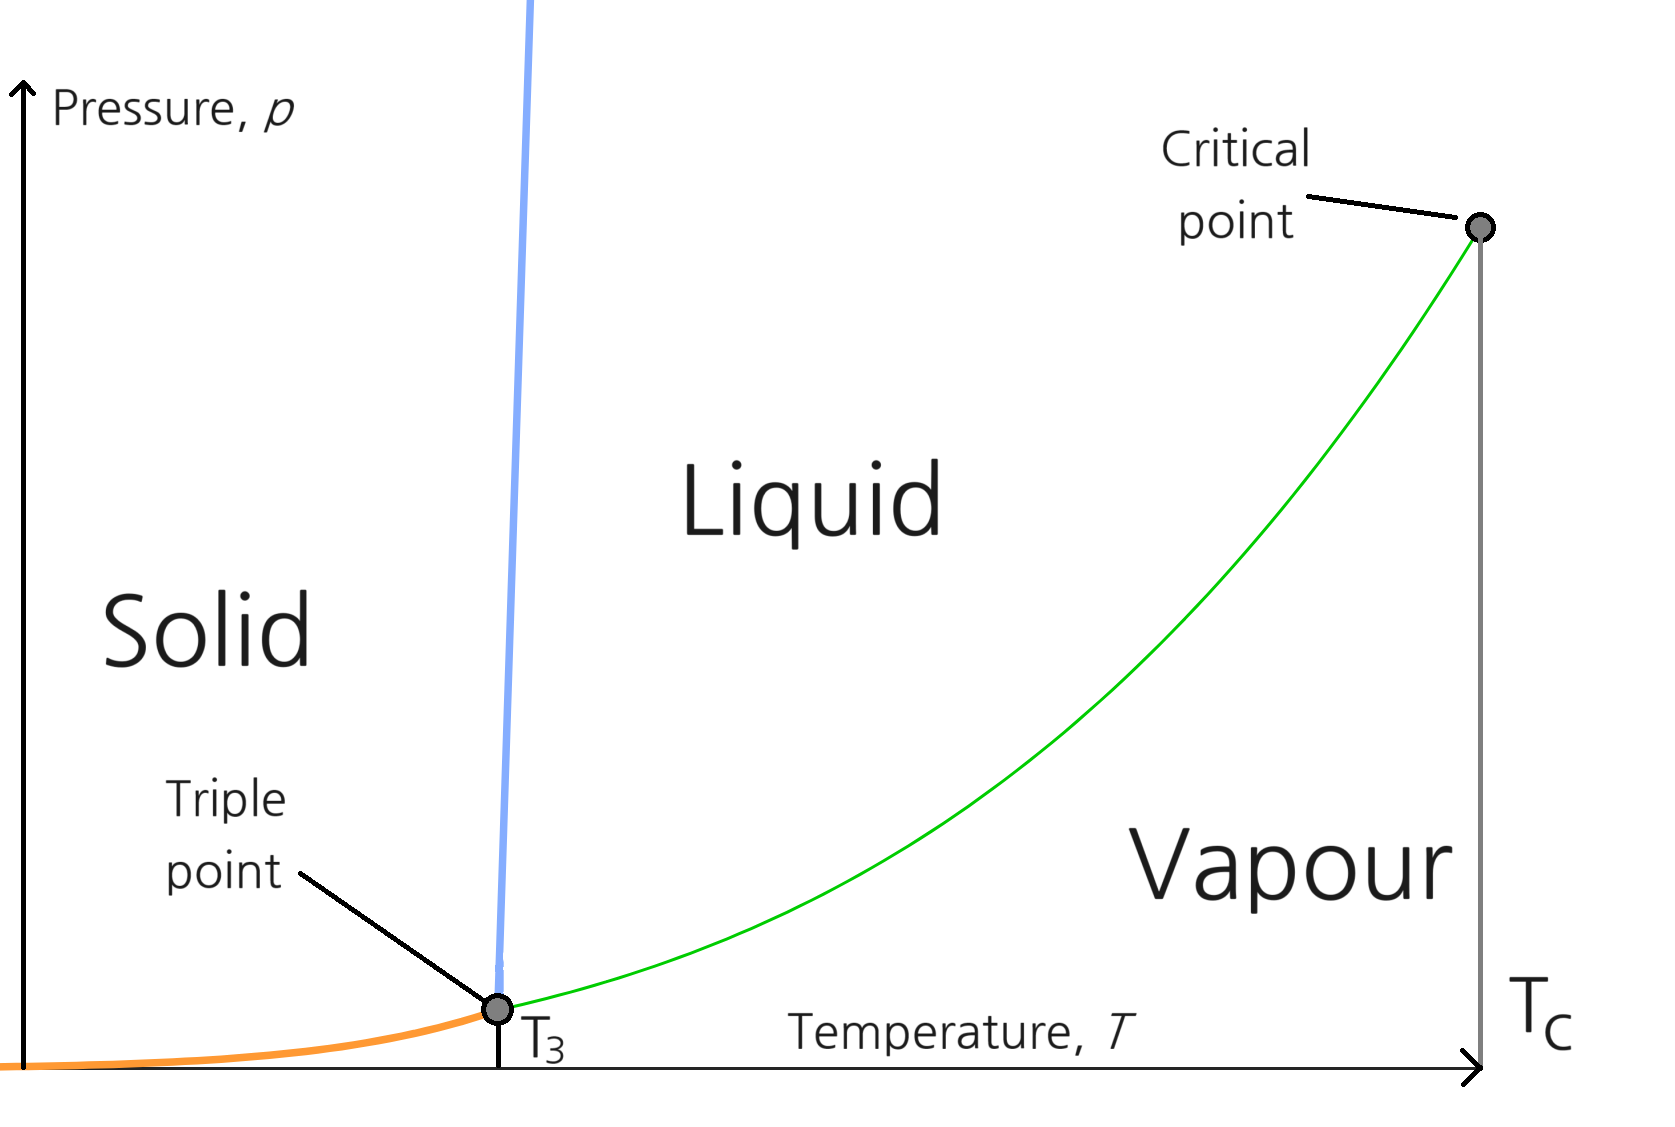
\includegraphics[scale=0.4]{Images/PhaseDiag1}
            \caption{상평형도}\label{f5}
        \end{figure}
        액체 상태의 물질은 \textbf{증기 압력(Vapour pressure)}을 가지며, 따라서 액체-기체 사이의 상 경계는 주어진 온도에서 증기 압력을 나타낸다. 
        마찬가지로, 고체-기체 상 경계는 주어진 온도에서 \textbf{승화 증기 압력(Sublimation vapour pressure)}을 나타낸다.
        \begin{defn}[액체-기체 사이의 논의]
        \begin{enum}
        \item 열린 용기에 액체가 담겨 있을 때, 외부 압력이 그 온도에서의 증기 압력보다 높다면 \textbf{증발(Vaporization, 기화라고도 함)}을 일으킨다. 
        \item 만약 외부 압력이 그 온도에서의 증기 압력과 같아진다면, 액체 전체에서 기화가 일어나는 \textbf{끓음(Boiling)}이라는 과정을 일으킨다. 
        \item 증기 압력이 외부 압력과 같아지는 지점을 \textbf{끓는점(Boiling point)}이라 한다.
        \item 외부 압력이 1 atm일 때의 끓는점을 \textbf{정상 끓는점(Normal boiling point, $T_b$)}이라 한다.
        \item 외부 압력이 1 bar일 때의 끓는점을 \textbf{표준 끓는점(Standard boiling point)}이라 한다. 일반적으로 표준 끓는점은 정상 끓는점보다 낮다.
        \end{enum}
        \end{defn}
        \begin{defn}[임계 상태와 관련한 서술]
        닫힌 용기에서 액체 상태의 물질을 가열하면 끓음이 일어나지 않는다. 대신 증기 압력이 증가하면서, 기체와 액체의 경계면이 사라지는 지점이 
        나타난다. 이때의 온도를 \textbf{임계 온도(Critical temperature, $T_c$)}라 하고, 임계 온도에서의 증기 압력을 \textbf{임계 압력(Critical pressure, $p_c$)}이라 
        한다. 이 지점 이상의 온도를 가지게 되면 물질은 하나의 균일한 상인 \textbf{초임계 유체(Supercritical fluid)}를 이룬다.
        \end{defn}
        \begin{defn}[고체-액체 사이의 논의]
        \begin{enum}
        \item 특정 압력에서 액체와 고체가 공존하면서 평형을 이루는 온도를 \textbf{녹는점(Melting temperature)}이라 한다. 
        \item 녹는점은 \textbf{어는점(Freezing temperature)}과 같다. 
        \item 1 atm에서의 어는점을 \textbf{정상 어는점(Normal freezing point, $T_f$)}이라 한다.
        \item 1 bar에서의 어는점을 \textbf{표준 어는점(Standard freezing point)}이라 한다. 
        대부분의 물질에서는 정상 어는점과 표준 어는점이 거의 일치한다. 정상 어는점은 \textbf{정상 녹는점(Normal melting point)}이라고도 한다.
        \end{enum}
        \end{defn}
        \begin{defn}[삼중점]
        세 개의 서로 다른 상이 공존하며 평형을 이루는 지점을 \textbf{삼중점(Triple point)}이라 한다. 이때의 온도를 $T_3$이라고도 나타낸다.
        \end{defn}
        순수한 물질의 삼중점은 변하지 않는다. 또한, 삼중점은 액체 상태의 물질이 존재할 수 있는 최소한의 압력에 해당한다. 또한, 고체-액체 상 경계의 
        기울기가 양수일 경우, 삼중점은 액체 상태의 물질이 존재할 수 있는 최소한의 온도에 해당한다. (예외로 물이 있다.)
        \par Josiah Willard Gibbs는 \textbf{상 규칙(Phase rule)}을 유도하였다. 각각의 변수들은 다음과 같다:
        \begin{enum}
            \item \textbf{변수(Variance, $F$)}는 자유도를 의미하며, 평형을 이루는 상의 개수를 바꾸지 않는 조건에서 자유로이 바꿀 수 있는 세기 성질의 개수를 나타낸다.
            \item \textbf{구성 성분(Constituent)}은 계를 구성하는 모든 화학종이다.
            \item \textbf{구성 요소(Component)}는 계를 구성하는 \textit{화학적으로 독립적인} 구성 성분이다.
            \item $C$는 구성 요소의 개수로, 계의 모든 상을 나타낼 수 있는 최소한의 구성 요소의 개수를 나타낸다.
        \end{enum}
        \par 먼저, 온도와 압력에 대한 자유도 2에서 시작한다. 이때 C개의 구성 요소가 있으면, 몰 분율이라는 요인에 의해 자유도가 제약된다. 
        $x_A + x_B + \cdots + x_J = 1$이므로, 구성 요소에 대해 $C-1$의 자유도가 주어진다. 이때 각 구성 요소에 대해 $P$만큼의 상이 가능하므로, 
        이 단계에서 가능한 자유도는 $P\left(C-1\right)+2$이다.
        \par 이제 평형 상태를 생각하자. $P$개의 상이 평형을 이룰 때, 화학 퍼텐셜은 $P$개의 상 모두에서 같아야 한다. 따라서 이때 감소되는 
        자유도는 $P-1$이고, $C$개의 구성 요소에 대해 이러한 자유도가 모두 감소되므로 가능한 자유도는 $P\left(C-1\right)-C\left(P-1\right) + 2$, 즉 
        $F = C - P + 2$를 만족한다.
        \par 따라서 Gibbs의 상 규칙은 다음과 같다:
        \begin{law}[상 규칙]
        \begin{equation*}
            F = C- P +2
        \end{equation*}
        \end{law}
        만약 구성 요소가 하나일 경우($C=1$), $F = 3-P$를 만족한다. 따라서 이때에는 상이 하나일 때 독립변수는 두 개, 상이 두 개일 때 독립변수는 하나, 
        상이 세 개(삼중점)일 때 독립변수는 없다. 이를 계가 \textbf{불변(Invariant)}이라 한다. 
        추가적으로, 구성 요소가 하나일 경우에는 네 개의 상이 공존하면서 평형을 이루는 점은 존재할 수 없다.
        \par \ref{phasethermo}에서 다루겠지만, 물을 비롯한 몇몇 물질에서는 고체-액체 상 경계의 기울기가 음수로 나타난다. 특히 물에서는 얼음 I 상의 빈 공간이 
        물일 때보다 많기 때문에 액체에서 얼음 I로 응고되면 부피가 증가한다. 또한, 헬륨-4의 경우 액체 상태가 2종류 존재한다. 이 두 액체의 $\displaystyle C_{p,m}$을 비교하면 불연속점이 
        나타난다. 이를 람다-상태 변화($\lambda$-transition)라 한다. 헬륨-II 액체 상태의 경우 \textbf{초유체(Superfluid)} 상태로, 점성이 0인 특성을 보인다.
    \section{상의 열역학적 관점}\label{phasethermo}
        \hspace{\parindent} 다음이 성립함은 \ref{dudhdadg}에서 살펴보았다:
        \begin{equation*}
            \difform G = V\difform p-S\difform T
        \end{equation*}
        각각에서, $\mu = G_m$이라는 사실을 이용하면 다음이 성립한다:
        \begin{equation*}
            \begin{aligned}
                \left(\frac{\partial \mu}{\partial T}\right)_p &= -S_m \\
                \left(\frac{\partial \mu}{\partial p}\right)_T &= V_m
            \end{aligned}
        \end{equation*}
        이때, $T>0$이면 $S_m>0$이므로, 온도가 증가할수록 화학 퍼텐셜은 감소한다. 
        일반적으로 $S_m\left(\mathrm{g}\right)>S_m\left(\mathrm{l}\right)>S_m\left(\mathrm{s}\right)$이므로, 화학 퍼텐셜의 기울기의 절댓값은 
        고체에서보다 액체에서, 액체에서보다 기체에서 더 크다.
        \par 또한, $V_m>0$에서 압력이 증가하면 화학 퍼텐셜은 증가한다. 대부분의 경우에서, $V_m\left(\mathrm{l}\right)>V_m\left(\mathrm{s}\right)$이므로 
        압력이 증가할 때 화학 퍼텐셜이 증가하는 정도는 고체에서보다 액체에서가 더 크다. 따라서 이 경우 압력이 증가하면 어는점이 올라간다. 
        그러나 물과 같은 일부 경우에서는 $V_m\left(\mathrm{l}\right)< V_m\left(\mathrm{s}\right)$이므로, 
        압력이 증가할 때 화학 퍼텐셜이 증가하는 정도는 액체에서보다 고체에서가 더 크다. 따라서 이 경우 압력이 증가하면 어는점이 내려간다.
        \par 액체나 고체 등에 비활성 기체(Inert gas)를 이용하여 압력을 가했을 때, 압력을 받는 물체의 증기 압력은 증가한다. 따라서 
        \textbf{부분 증기 압력(Partial vapour pressure)}을 정의할 수 있고, 이는 전체 압력 $P$와 관련이 있다. 
        위에서 언급한 것과 같이, $\displaystyle\left(\frac{\partial \mu}{\partial p}\right)_T = V_m$이 성립하므로, 증기를 이상 기체로 가정하면 
        $\displaystyle\difform \mu = V_m \difform p = RT \difform p /p$가 성립한다. 또한, 증기와 응축 상태(액체로 가정하겠다)가 평형을 이루므로, 다음이 성립한다: 
        $$
        \difform \mu\left(\mathrm{l}\right) = V_m\left(\mathrm{l}\right)\difform p 
        = \difform \mu\left(\mathrm{g}\right) = \frac{RT \difform p}{p}
        $$
        따라서, \underline{이때 불활성 기체는 증기와 상호작용하지 않고 액체에 녹지 않는다고 가정하면}\footnote[12]{%
        이 가정이 없을 경우 굉장히 복잡해진다.}, 정상 증기 압력 $p^\ast$와 액체에 추가로 가해진 압력 $\Delta P$에 대해 $p^\ast + \Delta p = p$라 
        가정할 때, 다음이 성립한다(단 이때 적분변수는 $p^\prime$으로 한다):
        \begin{equation*}
            RT \int_{p^\ast}^{p}\frac{\difform {p^\prime}}{p^{\prime}} = \int_{p^\ast}^{p^\ast + \Delta P}V_m\left(\mathrm{l}\right)\difform P
        \end{equation*}
        따라서 다음이 성립한다:
        \begin{equation*}
            \ln{\frac{p}{p^\ast}}=\frac{V_m\left(\mathrm{l}\right)}{RT}\Delta P
        \end{equation*}
        즉 $p=p^\ast e^{V_m\left(\mathrm{l}\right)\Delta P/RT}$가 성립한다.
        \par 상 $\alpha$와 상 $\beta$가 압력 $p$, 온도 $T$에서 평형을 이룰 때, 이 둘의 화학 퍼텐셜 $\mu$가 같음은 위에서 살펴보았다. 
        이제 상 경계의 기울기를 구할 것이다. $\mu = G_m$이라는 사실로부터 출발하자. 
        $\difform G_m = V_m \difform p - S_m \difform T$에서, 
        \begin{equation*}
            V_m \left(\alpha\right)\difform p - S_m \left(\alpha\right)\difform T = V_m \left(\beta\right)\difform p - S_m \left(\beta\right)\difform T
        \end{equation*}
        이 성립한다. 따라서 
        \begin{equation*}
            \left\{S_m\left(\beta\right) - S_m\left(\alpha\right)\right\}\difform T = \left\{V_m\left(\beta\right) - V_m\left(\alpha\right)\right\}\difform p
        \end{equation*}
        가 성립하고, 이를 정리하면 다음과 같다:
        \begin{equation*}
            \Delta_\mathrm{trs} S \difform T = \Delta_\mathrm{trs}V\difform p
        \end{equation*}
        따라서 다음과 같은 \textbf{Clapeyron 등식(Clapeyron equation)}을 유도할 수 있다:
        \begin{law}[Clapeyron 등식]
        \begin{equation*}
            \frac{\difform p}{\difform T} = \frac{\Delta_\mathrm{trs}S}{\Delta_\mathrm{trs}V}
        \end{equation*}
        \end{law}
        압력이 변화하는 조건에서는 각각의 "역수"를 취하면 된다.
        \par 식 \ref{trsentr}에 의해, 고체-액체 상 경계에서도 다음이 성립한다:
        \begin{equation*}
            \frac{\difform p}{\difform T} = \frac{\Delta_\mathrm{fus}H}{T \Delta_\mathrm{fus}V}
        \end{equation*}
        따라서 $\difform T$를 우변으로 넘기고 양변을 적분하면 다음과 같다:
        \begin{equation*}
            \int_{p^\ast}^{p}\difform p = \frac{\Delta_\mathrm{fus}H}{\Delta_\mathrm{fus}V}\int_{T^\ast}^{T}\frac{\difform T}{T}
        \end{equation*}
        따라서 다음이 성립한다:
        \begin{equation*}
            p = p^\ast + \frac{\Delta_\mathrm{fus}H}{\Delta_\mathrm{fus}V}\ln{\frac{T}{T^\ast}}
        \end{equation*}
        이때 $\displaystyle \ln{\frac{T}{T^\ast}} = \ln{\left(1+\frac{T-T^\ast}{T^\ast}\right)}\approx \frac{T-T^\ast}{T^\ast}$으로 근사할 수 있으므로, 
        다음과 같이 일차식으로 근사할 수 있다:
        \begin{equation*}
            p = p^\ast + \frac{\Delta_\mathrm{fus}H}{T^\ast \Delta_\mathrm{fus}V}\left(T-T^\ast \right)
        \end{equation*}
        \par 액체-기체 상 경계에서도 비슷하게 성립한다. 이때 기체의 부피가 액체의 부피보다 현저히 크기 때문에, $\Delta_\mathrm{vap}V \approx V_m\left(\mathrm{g}\right)$로 
        근사할 수 있다. 증기를 이상 기체로 근사하면, $V_m = RT/p$에서 
        $$
        \frac{\difform p}{\difform T} = \frac{\Delta_\mathrm{vap}H}{RT^2 /p}=\frac{p\Delta_\mathrm{vap}H}{RT^2}
        $$
        가 성립한다. 다시 정리하면 다음과 같은 \textbf{Clausius-Clapeyron 등식(Clausius-Clapeyron equation)}이 성립한다:
        \begin{law}[Clausius-Clapeyron 등식]
        \begin{equation*}
            \frac{\difform \ln{p}}{\difform T} = \frac{\Delta_\mathrm{vap}H}{RT^2}
        \end{equation*}
        \end{law}
        이 등식을 적분하면 다음과 같은 식 또한 성립한다:
        \begin{equation*}
            \ln{\frac{p}{p^\ast}} = -\frac{\Delta_\mathrm{vap}H}{R}\left(\frac{1}{T} - \frac{1}{T^\ast}\right)
        \end{equation*}
        \par 고체-기체 상 경계에서도 같은 과정을 통해 기울기를 구할 수 있다.